Este ensayo se realizó con el objetivo de medir la potencia de salida del amplificador utilizado en los dos puntos anteriores. La potencia fue medida para las condiciones de resistencia de carga igual a la impedancia de salida y máxima excursión simétrica de la tensión de salida. Ver fundamentos de este experimento en la sección \ref{sec:MaxPot}, del Marco Teórico.

Una de las formas más comunes de expresar el valor de la potencia de salida de un amplificador es en \textbf{dBm}, el cual es una unidad de medida de relación o razón de potencia expresada en decibelios con referencia a 1mW. Se puede obtener su valor a partir de la expresión \ref{eq::PotConVolReferidoa775mV} (Marco Teórico).

La forma más sencilla de determinar la \textbf{dBm} es mediante el empleo de instrumentos que posean escalas trazadas en \textbf{dB}, como lo es el multímetro analógico de la marca UNIVO.
Este instrumento no tiene la funcionalidad de medir potencia, pero se la puede medir indirectamente a partir de la medición de la tensión en la carga $R_{C1}$ en escala de decibeles. Como se explicó en el apartado \ref{sec:Gan} del marco teórico, por lo general la tensión se mide en la unidad de \textbf{dBu} (decibelios referidos a 0.775V).

Para esto, se dispuso los instrumentos de la misma forma que en la experiencia 1, conectando la carga $R_{C1}$ y moviendo la perilla hasta lograr el valor de resistencia igual a la impedancia de salida, el cual es de $ Z_o = 46.1 \pm 0.869  ~\Omega$.

Lo siguiente fue configurar el multímetro en la escala de decibeles, que está trazada
en el rango de 3V, y se procedió a conectar los terminales del multímetro a una tensión fija de 0.775V para poder calibrar el punto de 0 decibelios. 

\subsubsection{Mediciones}

Una vez terminada la calibración, se conectaron los terminales en paralelo con la resistencia de carga $R_{C1}$ para medir la caída de tensión. Para esta medición, el voltímetro estaba configurado para medir corriente alterna y además las puntas estaban conectadas una al borne común del multímetro y la otra a la terminal OUTPUT.

El resultado de la medición se visualiza en la figura \ref{fig:VoltajeDeSalidaDBu}.

\begin{equation}
    V_{dBu} = 8.20 \mathrm{dBu}
\end{equation}


\begin{figure}[H]
    \centering
    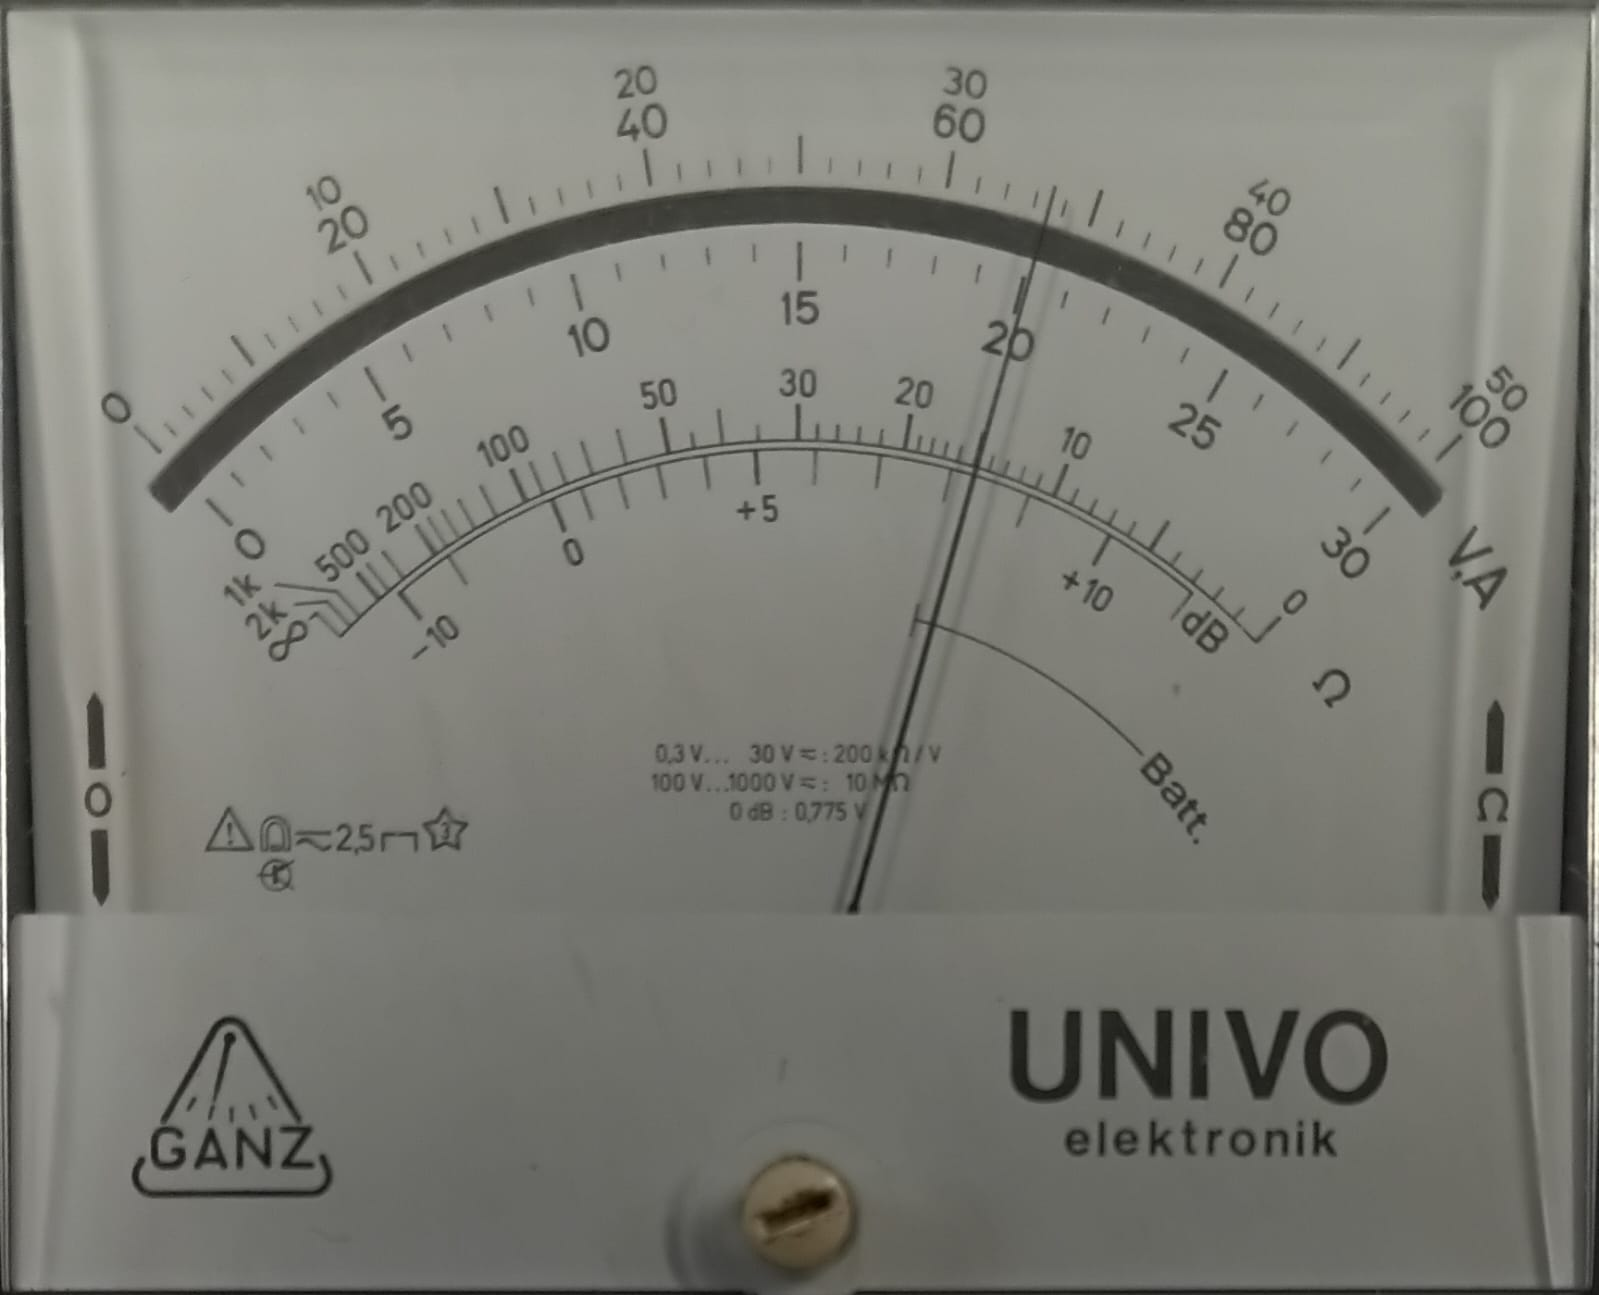
\includegraphics[width=0.45\linewidth]{Imagenes/dBuSal.jpeg}
    \caption{Voltaje de Salida en dBu}
    \label{fig:VoltajeDeSalidaDBu}
\end{figure}

Este valor en dBu obtenido es el primer término de la ecuación \ref{eq::PotConVolReferidoa775mV}, al cual se le debe sumar el término correspondiente a la resistencia sobre la que se midió ese voltaje. Por lo tanto, usando la ecuación, se obtiene que:

\begin{equation}
    P_{dBm} = V_{dBu} + 10\cdot\log{\frac{600\Omega}{R_x}}
\end{equation}

Reemplazando $V_{dBu}$ por el valor medido, y $R_x$ por la resistencia $R_{C1}$ sobre la cual se midió:

\begin{align}
    P_{dBm} =& 8.20 \mathrm{dB} + 10\cdot\log{\frac{600\Omega}{46.1\Omega}}
    \\ =& 8.20 \mathrm{dB} + 11.14 \mathrm{dB}
    \\ =& 19.34 \mathrm{dB}
\end{align}

\subsubsection{Comprobación}

Se puede comprobar la exactitud de este valor, calculando la potencia sobre la resistencia de salida y luego haciendo la conversión a \textit{dBm}. 

Para realizar este cálculo, tomaremos algunos datos del experimento 1: 

\begin{align*}
    v_s = 10,2 V_{pp} = 5,1 V_p
    \hspace{0.5cm}\longrightarrow \hspace{0.5cm}\text{En vacío}\\
    v_s'= 5,08 V_{pp} = 2,54 V_p 
    \hspace{0.5cm}\longrightarrow \hspace{0.5cm}\text{Con} ~R_{cl}=Z_o
\end{align*}

Ahora, se calculará la corriente eficaz $I_{ef}$ que circula por la resistencia $R_{cl}$.

\begin{equation*}
    I_{ef} = \cfrac{\cfrac{v_s}{\sqrt{2}}}{2 \cdot Z_o} 
    = \cfrac{\cfrac{2.54}{\sqrt{2}}}{2 \cdot 46.1} = 39.113 mA
    %\hspace{0.5cm} \Longrightarrow \hspace{0.5cm}
\end{equation*}

Entonces la potencia sobre la resistencia de carga en la salida será:

\begin{equation*}
    P = I_{ef} \cdot V_{ef}' = I_{ef} \cdot \cfrac{v_s'}{\sqrt{2}}
    = 39.113 \cdot 10^{-3} \cdot \cfrac{2.54}{\sqrt{2}} = 70.25 mW
\end{equation*}

Finalmente convertimos a dBm y comparamos resultados.

\begin{equation*}
    P_{dBm} = 10 \cdot \log \left( \cfrac{P}{1 mW} \right) = 10 \cdot \log \left( \cfrac{70.25 mW}{1 mW} \right) = 18.466 ~dBm
\end{equation*}

A primera vista parece un valor muy similar al obtenido en la medición, sin embargo cuando se transforma a mW el valor en dBm de la medición, se obtiene un valor de 85.9 mW, que está bastante alejado del valor calculado. 

Esta diferencia entre cálculo y medición, puede deberse a fallas en la calibración del instrumento para medir potencia y/o por falta de exactitud de este.
